\documentclass{article}

\usepackage[preprint]{neurips_2021}

\usepackage[utf8]{inputenc} % allow utf-8 input
\usepackage[T1]{fontenc}    % use 8-bit T1 fonts
\usepackage{hyperref}       % hyperlinks
\usepackage{url}            % simple URL typesetting
\usepackage{booktabs}       % professional-quality tables
\usepackage{amsfonts}       % blackboard math symbols
\usepackage{nicefrac}       % compact symbols for 1/2, etc.
\usepackage{microtype}      % microtypography
\usepackage{xcolor}         % colors

\usepackage{printlen}
\usepackage[pdftex]{graphicx}
\usepackage{lmodern}

\usepackage{pgf}

\title{Analysing Influential Factors\\of a Successful Movie}

\author{%
  Bálint Mucsányi\\
  Matrikelnummer 6013671\\
  \And
  Daniel Dauner\\
  Matrikelnummer 4182694\\
  \authorsmail
  \texttt{\{balint.mucsanyi, daniel-wilfried.dauner\}@student.uni-tuebingen.de} \\
}

\begin{document}

\maketitle

\begin{abstract}
  We use the official IMDb datasets extended with scraped content from the IMDb website to predict the IMDb rating based on features such as the length, budget, or genre of a movie. We use logistic regression for this purpose. Furthermore, we monitor the effect of COVID-19 on movie revenues in the form of a hypothesis test. %Furthermore, we monitor the effect of COVID-19 on revenues in the form of a hypothesis test. 
\end{abstract}

\section{Introduction}
The central question of our project was quite general: what factors affect the success of a movie? To be able to quantify the level of appreciation of the public towards a particular movie, we considered two indicators: the \emph{star rating} and the \emph{box-office gross}. To gather a representative dataset of films and their features, we used an extended version of the official IMDb dataset\footnote{\url{https://www.imdb.com/interfaces} (accessed on 14th January)}.

The IMDb website provides general information about movies, such as the runtime, the genre, or partially their budget and box-office gross.
The ratings of movies are aggregated by a weighted average and displayed on the title's main page. The exact method is not disclosed. According to IMDb~\cite{ratings}, the method detects and rates fraudulent votes differently.

In our first experiment, we studied the predictability of the IMDb rating of movies from various features with logistic regression.
More advanced techniques were applied to investigate the capability of logistic regression in comparison. Using a non-linear transformation on our labels, we also fit a linear regression model and compared it to the other two approaches.

In our second experiment, we examined the effect of the COVID-19 pandemic on movies that failed at the box office. We consider a movie as a box-office flop if its budget exceeds its worldwide gross. Using hypothesis tests, we show significant trends of the "Covid-year" 2020. We support our findings in code\footnote{\url{https://github.com/MucsanyiBalint/data_literacy_project}}. %All claims made are supported in code.\footnote{\url{https://github.com/MucsanyiBalint/data_literacy_project}}

\section{Data Collection}
IMDb offers a variety of datasets on their website that are refreshed daily. The datasets contained 598,851 data points labelled as movies, of which only 273,557 movies had a user rating. The following features were used for logistic regression and were directly provided by IMDb: release year, runtime, number of rating votes, and genre. Some features were not provided by the official data but were available on the titles' main page. We additionally collected the estimated budget, the worldwide box-office gross, the number of user reviews, and the number of critic reviews of all movies with a user rating using a web-scraper over the course of 200 hours. During scraping we only accessed data that were not part of IMDb's \verb"robots.txt" list. 

The dataset included financial features from various decades in several currencies. Consequently, we had to account for inflation and convert the values into a uniform currency. For that, we used the inflation data of 16 currencies~\cite{test}. Movies were discarded if no inflation rates were available for the given currency. Each financial feature was converted from the release year to the rate in January 2022. After that, all values were converted into USD based on exchange rates from the European Central Bank.

The categorical features of the dataset required additional preprocessing. IMDb considers 23 different genres. We decided to summarize these into 18 genres, due to a large amount of sparsely represented categories. Merging the numerous age restriction categories or creating useful meta-categories proved to be challenging, as the rating system is different for nearly every country. These also changed over time, resulting in a family of overlapping categories. Therefore, we only consider whether a movie has been rated or not.

Finally, we dropped any movies that did not have a complete set of features for the given experiment. The completed dataset consists of 10714 and 14674 movies for the movie rating prediction and the hypothesis test, respectively. As the hypothesis testing required fewer features, more movies were preserved.

\section{Prediction of Movie Rating}
In our first experiment, we chose the IMDb rating as the indicator of a film being cherished. We used 26 selected features, out of which 18 correspond to the \emph{genre} and one to whether the film was \emph{rated} or not. The remaining 7 were the \emph{release year}, the \emph{runtime}, the average \emph{rating}, the number of \emph{votes}, the \emph{budget}, the worldwide \emph{gross}, and the number of critic and user \emph{reviews}.

We used logistic regression to predict the IMDb rating of films based on the aforementioned covariates. The label in this case is a continuous value between 1 and 10. Thus, the output of the sigmoid non-linearity was further transformed to $\hat{y} = 9\cdot \sigma(\mathbf{\theta}^\top \mathbf{x}) + 1$. As the choice of the loss function was not immediately obvious, we experimented with the regular binary cross-entropy (BCE), the mean squared error (MSE), and the mean absolute error (MAE). For evaluation purposes and easier interpretability, we used MAE as our validation and test metric for all three approaches. We divided our dataset of 10714 samples with a 90\%-10\% split into training and test sets. A further 10\% of the training set was used for validation. We trained the models using steepest descent with a learning rate of $1e-3$. The results are summarized in Table~\ref{tab:losses}. The MSE variant achieves the lowest training and test error.

Surprisingly, according to the weights of the MSE logistic regression model, increasing the release year or the budget of a movie while keeping all other features fixed has a negative effect on its rating. Increasing the runtime, the number of votes, or the number of user reviews, however, shows a positive effect on the rating. The number of critic reviews and most categories have almost no effect. The importance of the covariates can not be determined even with a normalized dataset and the assumption of the model being correct, as some of them are rather correlated.

\begin{table}
  \caption{Final training and test losses of a logistic regression model trained with steepest descent using three different loss functions, and three deep ReLU networks. No notable differences of training and test error can be seen between different losses for logistic regression. The ReLU networks were trained with L2 regularization and early stopping. Test results for ReLU networks are not marginally better than using MSE logistic regression.}% (improvements are below 0.1 stars).}
  \label{tab:losses}
  \centering
  \begin{tabular}{lllllll}
    \toprule
    {} & \multicolumn{3}{c}{Logistic Regression} & \multicolumn{3}{c}{ReLU-Net}       \\
    \cmidrule(r){2-7}
    Variant              & MSE   & MAE    & BCE    & Depth-2 & Depth-4 & Depth-6 \\
    \midrule
    Final Training Loss  & 0.6023 & 0.5943 & 0.6079 & 0.5299  & 0.5211  & 0.5271  \\
    Test Loss            & 0.5980 & 0.5987 & 0.6086 & 0.5413  & 0.5454  & 0.5497  \\
    \bottomrule
  \end{tabular}
\end{table}

We also tried transforming the IMDb ratings to real numbers by using the inverse of the scaled and shifted sigmoid: $y^{(new)} = -\log\left(\frac{9}{y^{(old)} - 1} - 1\right)$. This made it possible to fit a linear regression model as well. The test loss, in this case, was $0.6012$, almost identical to the logistic regression variants.

Although all four approaches achieve a below-one-star MAE and there is an approximately linear relationship between most covariates and the label, we wanted to investigate whether a model with a non-linear decision boundary could achieve an even better generalization error. For this, we considered ReLU networks with varying depth, trained with MSE loss. The hidden layers contained 32 neurons each. The results are summarized in Table~\ref{tab:losses}. No architecture achieved a 0.1-star error improvement compared to MSE logistic regression.

We did not manage to considerably improve the accuracy of logistic regression by using deeper models. This could indicate that our covariates are not descriptive enough or are simply too noisy to go below the 0.5-0.6 test MAE regime. However, as our method and architecture selection was not by any means extensive, this remains to be a hypothesis. In the future, we would also like to experiment with kernel machines~\cite{10.1214/009053607000000677}.

\begin{figure}
    \begin{center}
        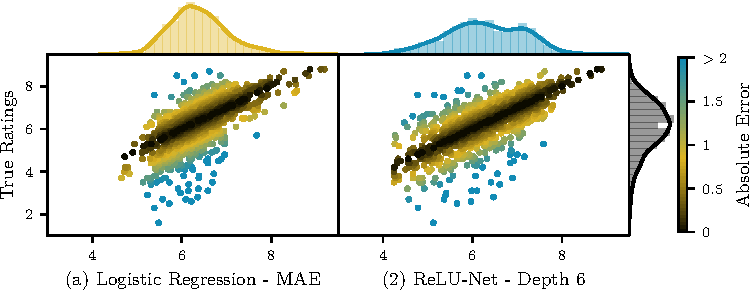
\includegraphics[width=.8\linewidth]{gfx/fig1.pdf}
    \end{center}
    \caption{Prediction map of MSE logistic regression and the largest ReLU-Net. Although logistic regression achieves a below-one-star MAE, it performs poorly outside of the $5-8$ rating range. The ReLU-Net has a similar error structure, with a slightly larger range where its predictions are mostly correct.}
\end{figure}

\section{Movie Industry in 2020}
In the second part of our study, we turned to the second indicator that a film is generally enjoyed by the public: the box-office gross. According to the Motion Pictures 2020 Theme Report~\cite{mp2020}, COVID-19 had a detrimental effect to the worldwide grosses. We wanted to verify this claim with our available data. For this, we used all movies in the IMDb database with available gross and budget and considered the frequency of flops in years preceding 2020 and in 2020, separately.

Our null hypothesis was that the number of flops in 2020 comes from the same distribution as in all preceding years. We considered a standard $\alpha = 0.05$ one-sided test, treating only more flops as extreme cases. The rationale behind this was that we wanted to study whether COVID-19 had a negative effect or not. In this case, $\emph{p-value} = \sum_{m = m_{2020}}^{N_{2020}} p(m \mid H_0)$, where $m_{2020}$ is the number of flops in 2020 and $N_{2020}$ is the number of all movies in 2020 with available gross and budget. As seen in the lecture, the distribution $p(m \mid H_0)$ in this case is beta-binomial, with parameters $N_{2020}, m_{<2020} + 1, N_{<2020} - m_{<2020} + 1$. Here $m_{<2020}$ is the number of flops before 2020, and $N_{<2020}$ is the number of movies before 2020. The results of the test can be seen in Figure~\ref{fig:hyp}.

Even though a significant result was obtained, one would also get a significant result for the years preceding 2020 as well. However, if \emph{p-values} are calculated for a fixed year for all possible year intervals [lower bound, year), 2020 is the first year since 2007 where the result is significant for $\emph{every possible interval}$. This highlights the year 2020 as an interesting outlier in the middle of an already significant trend of increasing flops in previous years.

\begin{figure}
    \begin{center}
        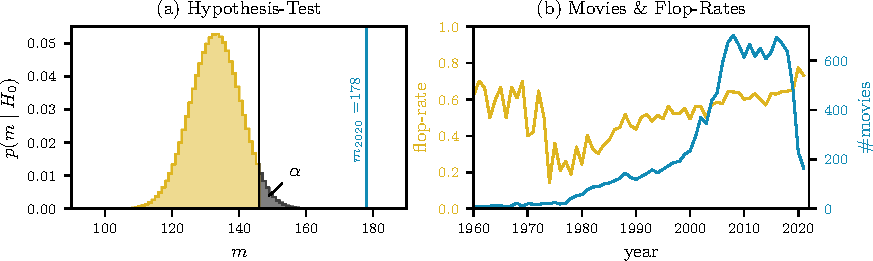
\includegraphics[width=\linewidth]{gfx/fig2.pdf}
    \end{center}
    \caption{(a) One-sided hypothesis test. The results are significant ($\emph{p-value} = 7.234\mathrm{e}{-10}$). (b) Number of movies (blue) and flops (yellow) plotted against years. In 2018-2021, a significant drop in the number of movies can be observed, with the number of flopping movies not dropping nearly as much in 2020.}
    \label{fig:hyp}
\end{figure}

In our last experiment, we connected the two indicators of a successful movie we considered: the IMDb rating and the box-office gross. We divided our dataset into two parts: one with an IMDb rating less than $5$ (bad movies), and one with greater than or equal to $5$ (good movies). We conducted the previous hypothesis test on the two datasets separately. The result for the bad movies was not significant ($\emph{p-value} = 0.1962$), thus we cannot state that the rate of flopping for bad movies changed based on this test. Conversely, the results for the good movies is significant ($\emph{p-value} = 4.4533\mathrm{e}{-9}$). Based on this test, we can conclude that COVID-19 also greatly affected the success-rate of highly rated movies with high probability.

\section{Conclusion}
To answer the question "What factors affect the success of a movie?", we considered two metrics: the IMDb rating and the box-office gross. In our first experiment, we studied the predictability of the IMDb rating from several features of a movie. According to the weights of MSE logistic regression, increasing the release year or the budget of a movie had a negative effect on the rating, whereas increasing the runtime, the number of votes, or the number of user reviews improved it.

In the second experiment, we studied the effects of COVID-19 on the worldwide gross of movies. The test showed significant results in the number of flops for 2020 compared to all previous years. To connect the two indicators, we divided our dataset based on the IMDb rating and conducted two separate tests. A significant result was only obtained for good movies, showing that apart from the features of logistic regression, COVID-19 also greatly affected the success of good movies.

\bibliographystyle{plain}
\bibliography{bib}
\end{document}
